\documentclass[11pt,a4paper]{article}

\usepackage[margin=22mm]{geometry}
\usepackage{array}
\usepackage{booktabs}
\usepackage{longtable}
\usepackage{enumitem}
\usepackage{xcolor}
\usepackage{graphicx}
\usepackage{float}
\usepackage{listings}
\usepackage{tikz}
\usepackage{hyperref}
\usetikzlibrary{arrows.meta,positioning,shapes.geometric}

\hypersetup{
  colorlinks=true,
  linkcolor=blue!50!black,
  urlcolor=blue!50!black,
  citecolor=blue!50!black,
  pdftitle={ADC Temperature Monitor Project Documentation},
  pdfauthor={ADC Project}
}

\lstset{
  basicstyle=\ttfamily\small,
  breaklines=true,
  columns=fullflexible,
  frame=single,
  framerule=0.3pt,
  rulecolor=\color{black!35},
  backgroundcolor=\color{black!3}
}

\tikzset{
  block/.style={
    draw,
    rounded corners=2pt,
    align=center,
    minimum height=8mm,
    text width=28mm,
    fill=blue!5
  },
  wideblock/.style={
    draw,
    rounded corners=2pt,
    align=center,
    minimum height=8mm,
    text width=38mm,
    fill=blue!5
  },
  hwblock/.style={
    draw,
    rounded corners=2pt,
    align=center,
    minimum height=8mm,
    text width=30mm,
    fill=green!7
  },
  faultblock/.style={
    draw,
    rounded corners=2pt,
    align=center,
    minimum height=8mm,
    text width=31mm,
    fill=red!7
  },
  every edge/.style={draw, -{Latex[length=2.4mm]}, line width=0.45pt}
}

\title{ADC Temperature Monitor\\\large STM32L476RG Internal Sensor, ADC1, DMA, MFS Display, and UART Product Documentation}
\author{Project documentation staged in \texttt{docs/}}
\date{May 14, 2026}

\begin{document}
\maketitle
\tableofcontents
\newpage

\section{Executive Summary}

This project is a bare-metal CMSIS firmware product for the NUCLEO-L476RG board.
From the outside, the product behaves as a compact temperature monitor:

\begin{itemize}[leftmargin=*]
  \item It powers from the Nucleo board USB/ST-LINK path.
  \item It samples the STM32L476RG internal temperature sensor and internal voltage reference.
  \item It compensates the temperature reading against the measured analog supply.
  \item It displays the rounded temperature on a four-digit Multi-Function Shield display.
  \item It emits one diagnostic line per second through the ST-LINK virtual COM port.
\end{itemize}

The implementation is intentionally small. Hardware-facing side effects live in the
driver modules under \texttt{src/}; the foreground application in \texttt{main.c}
only sequences reads, display refresh, and serial reporting.

\section{Source of Truth}

The documentation is derived from the local firmware plus official
STMicroelectronics documents:

\begin{itemize}[leftmargin=*]
  \item Local firmware: \texttt{src/main.c}, \texttt{src/temp\_sensor.c},
        \texttt{src/mfs\_display.c}, \texttt{src/debug\_uart.c}, and
        \texttt{src/timebase.c}.
  \item UM1724, \emph{STM32 Nucleo-64 boards (MB1136)}, official ST user
        manual: \url{https://www.st.com/resource/en/user_manual/um1724-stm32-nucleo64-boards-mb1136-stmicroelectronics.pdf}.
  \item MB1136-DEFAULT-C03 official board schematic:
        \url{https://www.st.com/resource/en/schematic_pack/mb1136-default-c03_schematic.pdf}.
  \item STM32L476xx official datasheet:
        \url{https://www.st.com/resource/en/datasheet/stm32l476re.pdf}.
\end{itemize}

Official document pages consulted for hardware evidence include the
NUCLEO-L476RG Arduino connector table in UM1724 and sheet 3 of the MB1136
schematic, where the STM32 pin mapping, AVDD, USART pins, and Arduino digital
signals are visible. The official PDFs are staged locally under
\texttt{docs/source-of-truth/}; the screenshots in
Section~\ref{sec:official-hardware-evidence} are raster extracts from those
documents. Project-specific diagrams are rendered as vector figures in this
report.

\section{Repository and Build Context}

\begin{longtable}{>{\raggedright\arraybackslash}p{0.28\linewidth}p{0.64\linewidth}}
\toprule
Item & Local project value \\
\midrule
\endhead
Core/domain path & \texttt{src/temp\_sensor.c}, \texttt{include/temp\_sensor.h} \\
Application/orchestration path & \texttt{src/main.c} \\
Display hardware adapter & \texttt{src/mfs\_display.c}, \texttt{include/mfs\_display.h} \\
Serial hardware adapter & \texttt{src/debug\_uart.c}, \texttt{include/debug\_uart.h} \\
Timing adapter & \texttt{src/timebase.c}, \texttt{include/timebase.h} \\
Build system & PlatformIO project, \texttt{platformio.ini} \\
Target board & \texttt{nucleo\_l476rg} \\
Framework & CMSIS \\
Compiler flags & \texttt{-Wall -Wextra -Wpedantic} \\
Tests path & \texttt{test/README}; no executable test suite is defined \\
Generated/vendor paths & \texttt{.pio/} build output is generated and should not be hand-edited \\
\bottomrule
\end{longtable}

Canonical build command from the project README:

\begin{lstlisting}[language=bash]
turn-signals/.venv/bin/pio run -d adc -e nucleo_l476rg
\end{lstlisting}

The current checkout does not contain that \texttt{pio} executable, and
\texttt{pio} is not on \texttt{PATH}. The existing \texttt{.pio/build/}
directory does contain prior firmware artifacts, but those artifacts are not a
replacement for a fresh build.

\section{Black-Box Product Contract}

\subsection{Inputs}

\begin{itemize}[leftmargin=*]
  \item Electrical power through the Nucleo board USB/ST-LINK path.
  \item The STM32L476RG die temperature, sensed internally by the MCU.
  \item The MCU internal bandgap reference, \texttt{VREFINT}, used to infer the
        effective analog supply during conversion.
\end{itemize}

There is no external analog signal wired into this project. The ADC channels are
internal channels selected by firmware.

\subsection{Outputs}

\begin{itemize}[leftmargin=*]
  \item Four-character Multi-Function Shield display text:
        \texttt{NN C}, \texttt{-N C}, \texttt{AERR}, or \texttt{DERR}.
  \item USART2 diagnostic line through the ST-LINK virtual COM port at
        115200 baud.
\end{itemize}

Successful serial output has this contract:

\begin{lstlisting}
adc-temp status=OK raw_temp=<adc_code> raw_vref=<adc_code> vdda_mv=<millivolts> temp_c=<signed_decimal_celsius>
\end{lstlisting}

Fault output has this contract:

\begin{lstlisting}
adc-temp status=ERR adc_fault=<0_or_1> dma_fault=<0_or_1>
\end{lstlisting}

\section{Hardware Architecture}

\subsection{Board and MCU}

The target is the NUCLEO-L476RG board with an STM32L476RG microcontroller. UM1724
identifies the Nucleo-64 board family as Arduino Uno V3 compatible and exposes
the STM32 pins through Arduino headers and ST morpho headers. The firmware uses
these board-level connections:

\begin{longtable}{>{\ttfamily}p{0.16\linewidth}>{\ttfamily}p{0.16\linewidth}p{0.52\linewidth}}
\toprule
Signal & STM32 pin & Use in this project \\
\midrule
\endhead
ADC1\_IN17 & internal & Internal temperature sensor analog signal. \\
ADC1\_IN0 & internal & VREFINT internal reference channel. \\
PA2 & USART2\_TX & ST-LINK virtual COM transmit path; Arduino D1 in UM1724. \\
PB5 & D4 & Multi-Function Shield latch pin in this firmware. \\
PA8 & D7 & Multi-Function Shield shift clock pin in this firmware. \\
PA9 & D8 & Multi-Function Shield shift data pin in this firmware. \\
AVDD & board analog supply & ADC reference domain used by the conversion result. \\
\bottomrule
\end{longtable}

The official MB1136 schematic shows the MCU sheet with PA2 labeled on the
USART transmit net, PB5 mapped to D4, PA8 mapped to D7, PA9 mapped to D8, and
VDDA/VREF+ tied into the analog supply domain through the board analog power
network. Those connections match the firmware constants in \texttt{debug\_uart.c}
and \texttt{mfs\_display.c}.

\subsection{ADC Signal Path}

The STM32L476xx datasheet describes the temperature sensor as an internal analog
source connected to ADC1 channel 17 and ADC3 channel 17. The same datasheet
describes VREFINT as an internal stable bandgap reference connected to ADC1
channel 0. The firmware selects ADC1 channel 17 followed by ADC1 channel 0 in
the regular conversion sequence.

\subsection{Display Interface}

The display driver is a bit-banged serial interface using three GPIO outputs:

\begin{itemize}[leftmargin=*]
  \item latch: PB5, Arduino D4
  \item clock: PA8, Arduino D7
  \item data: PA9, Arduino D8
\end{itemize}

Each display refresh writes two bytes: inverted seven-segment bits and a digit
select mask. The firmware multiplexes one digit every 2 ms, so each of four
digits is refreshed every 8 ms, approximately 125 Hz per digit.

\subsection{UART Interface}

USART2 transmit uses PA2 alternate function 7. UM1724 maps PA2 to Arduino D1
and USART2\_TX on the NUCLEO-L476RG connector table. The project uses transmit
only; PA3/USART2\_RX is not configured by this firmware.

\section{Firmware Architecture}

\subsection{Module Responsibilities}

\begin{longtable}{>{\ttfamily}p{0.25\linewidth}p{0.62\linewidth}}
\toprule
Module & Responsibility \\
\midrule
\endhead
main.c & Board boot sequencing, display refresh cadence, serial reporting cadence, and sleep between interrupts. \\
temp\_sensor.c & ADC1 and DMA1 Channel 1 setup, fault tracking, raw sample averaging, VDDA estimation, temperature calibration math. \\
mfs\_display.c & GPIO setup for display pins, seven-segment character encoding, shift-register writes, digit blanking. \\
debug\_uart.c & USART2 TX GPIO alternate function setup and blocking transmit helpers. \\
timebase.c & SysTick millisecond counter. \\
\bottomrule
\end{longtable}

\subsection{Initialization Sequence}

At boot, \texttt{main.c} executes:

\begin{enumerate}[leftmargin=*]
  \item \texttt{SystemCoreClockUpdate()} to synchronize CMSIS clock metadata.
  \item \texttt{mfs\_display\_init()} to configure the display GPIOs and blank the display.
  \item \texttt{timebase\_init()} to start SysTick at 1 kHz.
  \item \texttt{debug\_uart\_init(115200)} to enable the diagnostic channel.
  \item \texttt{temp\_sensor\_init()} to configure ADC1, DMA1 Channel 1, internal ADC channels, calibration, and continuous conversion.
\end{enumerate}

If ADC initialization fails, the serial channel reports a boot fault and the
display path remains capable of showing \texttt{AERR}.

\subsection{ADC and DMA Configuration}

\texttt{temp\_sensor\_init()} configures a continuous two-channel ADC scan:

\begin{itemize}[leftmargin=*]
  \item ADC common register enables the ADC clock mode, temperature sensor, and
        VREFINT path.
  \item ADC self-calibration is run before enabling ADC1.
  \item DMA1 Channel 1 reads from \texttt{ADC1->DR} into
        \texttt{g\_adc\_samples}.
  \item DMA memory increment and circular mode are enabled.
  \item DMA peripheral and memory width are halfword.
  \item The regular sequence length is two conversions:
        temperature sensor channel 17 and VREFINT channel 0.
  \item ADC continuous conversion, DMA, DMA circular request mode, and overrun
        overwrite mode are enabled.
\end{itemize}

The sample buffer stores 16 repeated scan pairs:

\[
N_{\mathrm{pairs}} = 16,\qquad
N_{\mathrm{channels}} = 2,\qquad
N_{\mathrm{samples}} = 32.
\]

For scan pair \(i\), the buffer layout is:

\[
x_{2i} = T_{\mathrm{raw},i},\qquad
x_{2i+1} = V_{\mathrm{REFINT},i}.
\]

\section{Measurement and Calibration Equations}

\subsection{Averaging}

The driver averages 16 raw samples for each channel:

\[
\overline{T}_{raw}
  = \frac{1}{16}\sum_{i=0}^{15}T_{\mathrm{raw},i},
\qquad
\overline{V}_{ref}
  = \frac{1}{16}\sum_{i=0}^{15}V_{\mathrm{REFINT},i}.
\]

The average is integer division in firmware. This intentionally trades fractional
precision for a simple fixed-point implementation with no floating-point runtime
dependency.

\subsection{Analog Supply Estimation}

ST stores a factory VREFINT calibration code measured at
\(V_{DDA,cal}=3000\,\mathrm{mV}\). The firmware reads that halfword from
\texttt{0x1FFF75AA}. Assuming the VREFINT physical voltage is stable, the ADC
code is inversely proportional to the active ADC reference voltage. The firmware
therefore estimates:

\[
V_{DDA}
  = \frac{3000 \cdot VREFINT_{CAL}}{\overline{V}_{ref}}
  \quad\mathrm{mV}.
\]

This is exactly the integer expression in \texttt{temp\_sensor.c}:

\[
\texttt{vdda\_mv}
  = \frac{\texttt{VREFINT\_CAL\_MV} \cdot \texttt{vref\_cal}}
         {\texttt{vref\_raw}}.
\]

\subsection{Temperature Code Compensation}

The ST temperature calibration points are measured at 3.0 V. The active
temperature ADC code is first normalized back to the 3.0 V calibration domain:

\[
T_{code,3.0V}
  = \frac{\overline{T}_{raw}\cdot V_{DDA}}{3000}.
\]

The firmware calls this value \texttt{temp\_corrected}.

\subsection{Two-Point Temperature Interpolation}

The STM32L476xx datasheet gives two factory calibration points:

\begin{itemize}[leftmargin=*]
  \item \texttt{TS\_CAL1} at address \texttt{0x1FFF75A8}, measured at 30 degrees C.
  \item \texttt{TS\_CAL2} at address \texttt{0x1FFF75CA}, measured at 110 degrees C.
\end{itemize}

The firmware computes centi-degrees Celsius by linear interpolation:

\[
T_{cC}
  =
  \left(
    \frac{(T_{code,3.0V} - TS_{CAL1})\cdot(110-30)\cdot100}
         {TS_{CAL2}-TS_{CAL1}}
  \right)
  + 30\cdot100.
\]

The public snapshot field \texttt{temp\_centi\_c} stores this signed fixed-point
result. For example, 2734 means 27.34 degrees C.

\section{Runtime Behavior}

\subsection{Main Loop Cadence}

The main loop is cooperative and time-triggered by the SysTick millisecond
counter:

\begin{longtable}{>{\raggedright\arraybackslash}p{0.22\linewidth}p{0.22\linewidth}p{0.44\linewidth}}
\toprule
Cadence & Constant & Action \\
\midrule
\endhead
2 ms & \texttt{REFRESH\_MS} & Scan the next display digit. \\
250 ms & \texttt{DISPLAY\_UPDATE\_MS} & Read latest ADC/DMA snapshot and refresh the display text buffer. \\
1000 ms & \texttt{SERIAL\_UPDATE\_MS} & Read latest snapshot and emit a UART diagnostic line. \\
\bottomrule
\end{longtable}

After each loop pass, the firmware executes \texttt{\_\_WFI()} and waits for the
next interrupt. SysTick wakes the loop for normal timing. ADC overrun also has an
interrupt path through \texttt{ADC1\_2\_IRQHandler()}.

\subsection{Fault Model}

The fault model is intentionally simple:

\begin{itemize}[leftmargin=*]
  \item ADC self-calibration timeout or ADC ready timeout sets \texttt{adc\_fault}.
  \item ADC overrun interrupt sets \texttt{adc\_fault}.
  \item DMA transfer error sets \texttt{dma\_fault}.
  \item A snapshot is valid only when the sample path has data and neither fault
        flag is set.
\end{itemize}

The display contracts are:

\begin{itemize}[leftmargin=*]
  \item \texttt{AERR}: ADC path is invalid or not ready.
  \item \texttt{DERR}: DMA transfer path reported a fault.
  \item \texttt{NN C} or \texttt{-N C}: valid rounded temperature, clamped to
        the display range from -9 to 99 degrees C.
\end{itemize}

\section{Connection Checklist}

\begin{longtable}{>{\ttfamily}p{0.16\linewidth}>{\ttfamily}p{0.18\linewidth}>{\raggedright\arraybackslash}p{0.48\linewidth}}
\toprule
Connection & Source evidence & Practical check \\
\midrule
\endhead
PA2 / USART2\_TX & UM1724 NUCLEO-L476RG connector table; MB1136 schematic & Serial terminal on ST-LINK VCP should receive one line per second at 115200 baud. \\
PB5 / D4 & UM1724 connector table; MB1136 schematic; \texttt{mfs\_display.c} & Display latch transitions during refresh. \\
PA8 / D7 & UM1724 connector table; MB1136 schematic; \texttt{mfs\_display.c} & Display clock toggles during refresh. \\
PA9 / D8 & UM1724 connector table; MB1136 schematic; \texttt{mfs\_display.c} & Display data changes before clock pulses. \\
ADC1 channel 17 & STM32L476xx datasheet; \texttt{temp\_sensor.c} & Raw temperature code appears in serial telemetry. \\
ADC1 channel 0 & STM32L476xx datasheet; \texttt{temp\_sensor.c} & Raw VREFINT code is nonzero; derived VDDA is plausible. \\
\bottomrule
\end{longtable}

\section{Official Hardware Evidence}
\label{sec:official-hardware-evidence}

The hardware claims in this report are tied to the official ST documents listed
in Section 2. The following screenshots are direct page renders from the staged
official PDFs. The explanation below each screenshot states exactly which
firmware claim the official page supports.

\subsection{NUCLEO-L476RG Arduino Connector Evidence}

\begin{figure}[H]
\centering
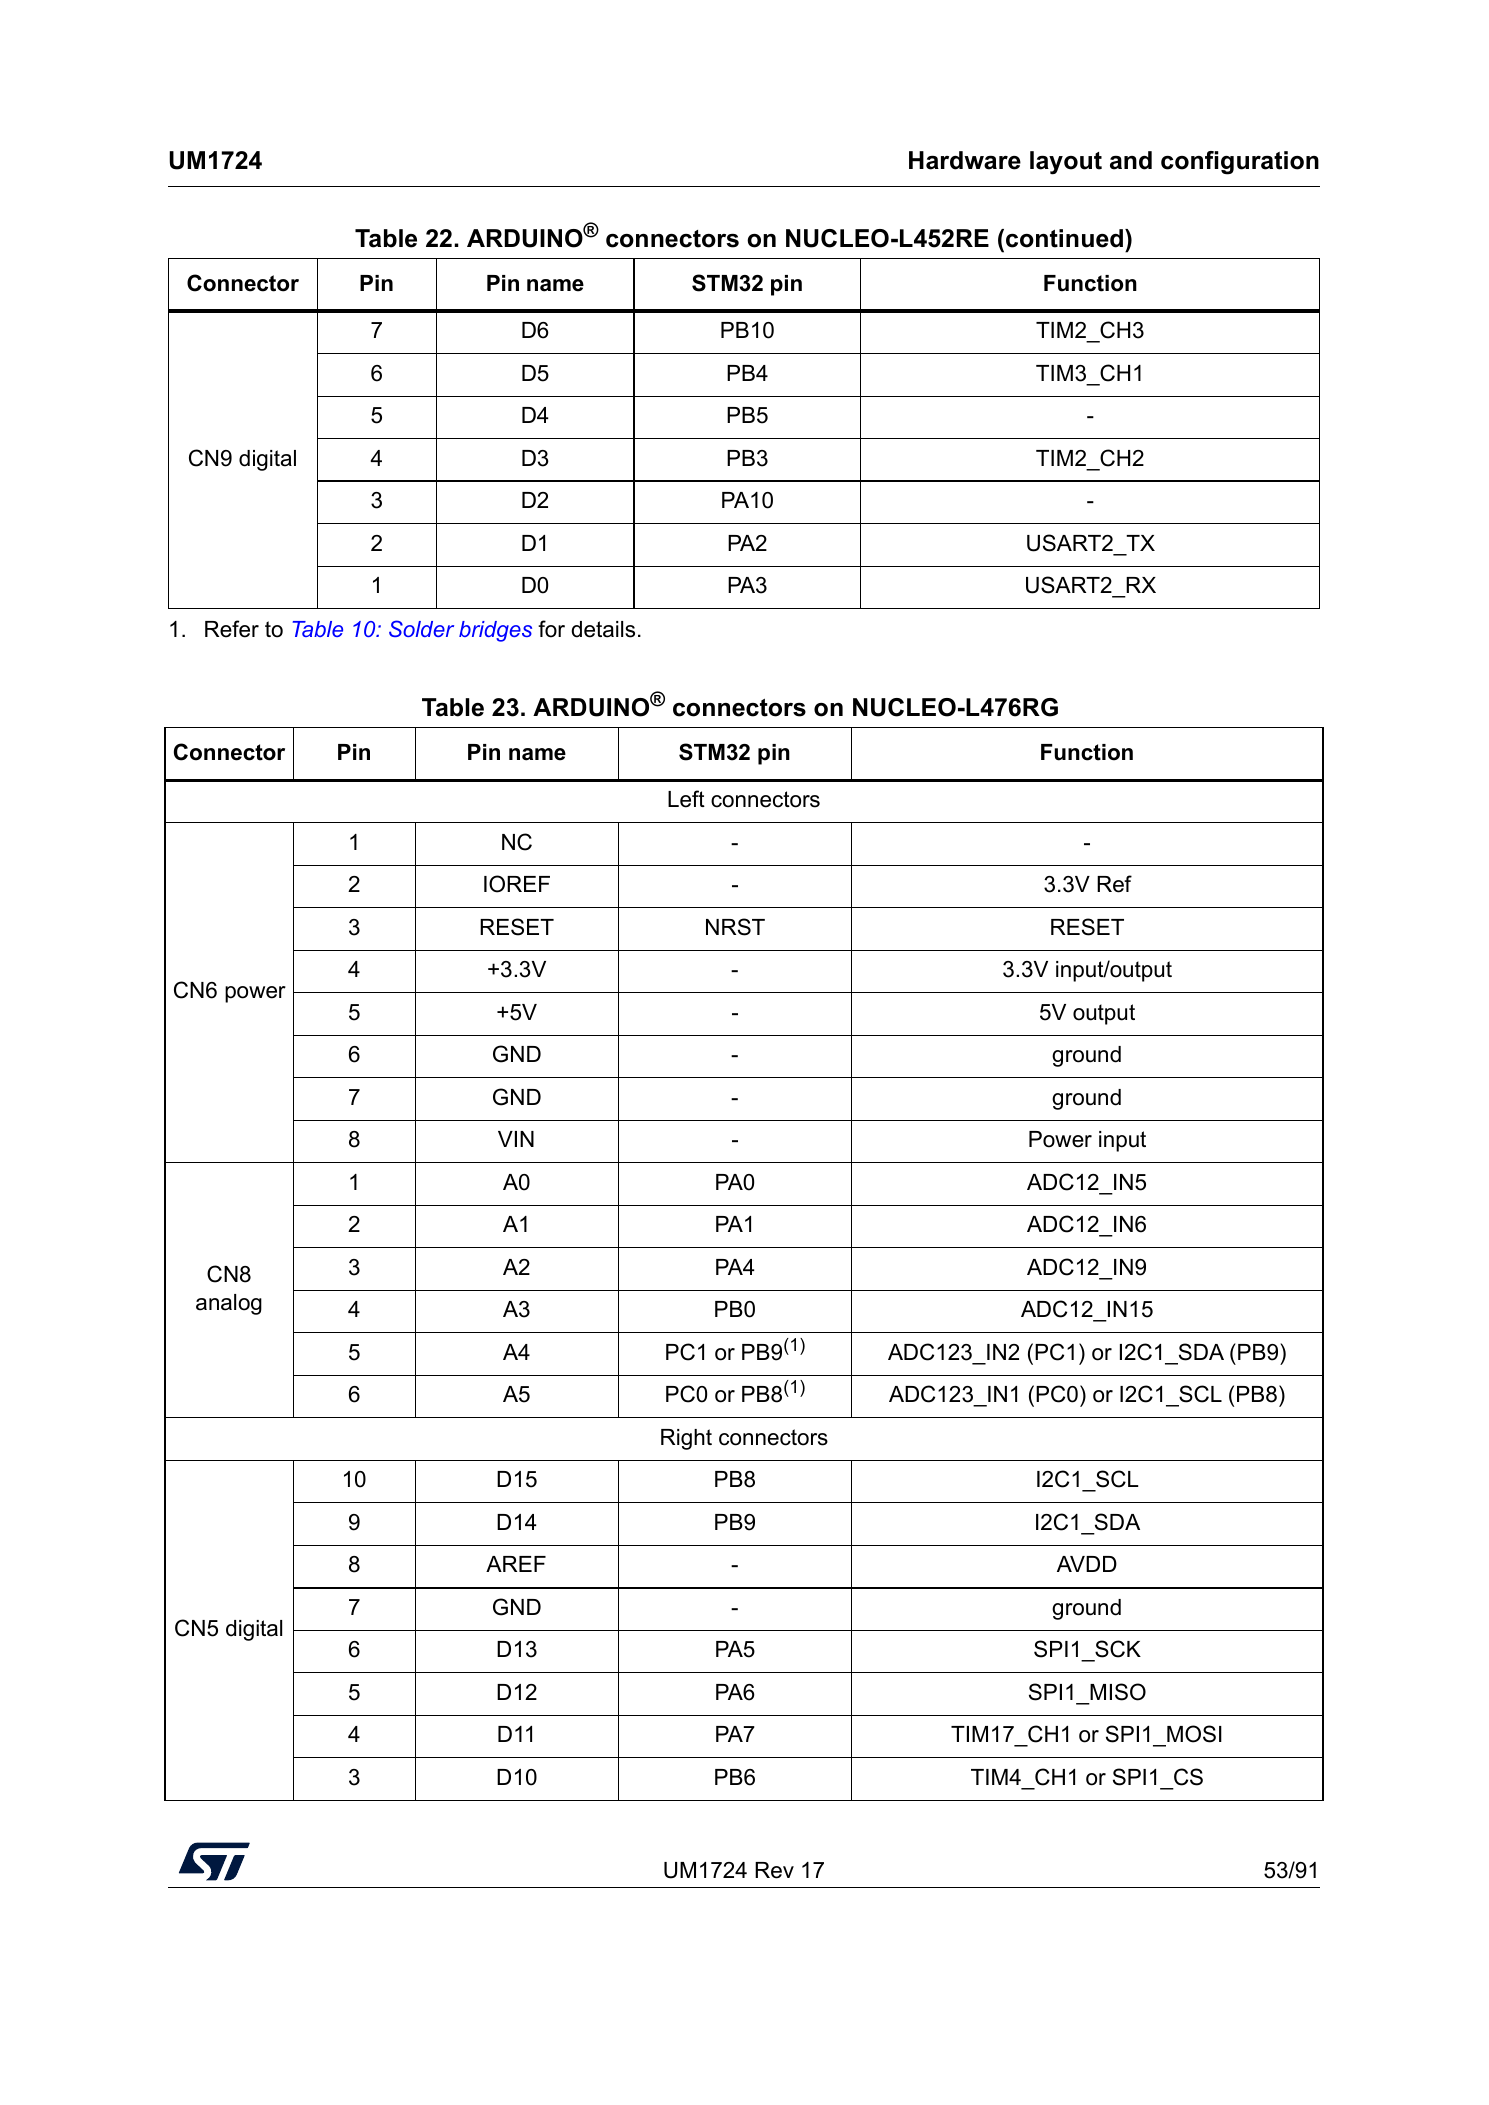
\includegraphics[width=0.94\linewidth]{assets/screenshots/um1724-table23-arduino-connectors-53.png}
\caption{UM1724 page 53, where Table 23 begins for the NUCLEO-L476RG Arduino
connectors. This page shows AREF as AVDD and begins the connector table used to
validate the board-level signal naming.}
\label{fig:official-um1724-table23-page53}
\end{figure}

\begin{figure}[H]
\centering
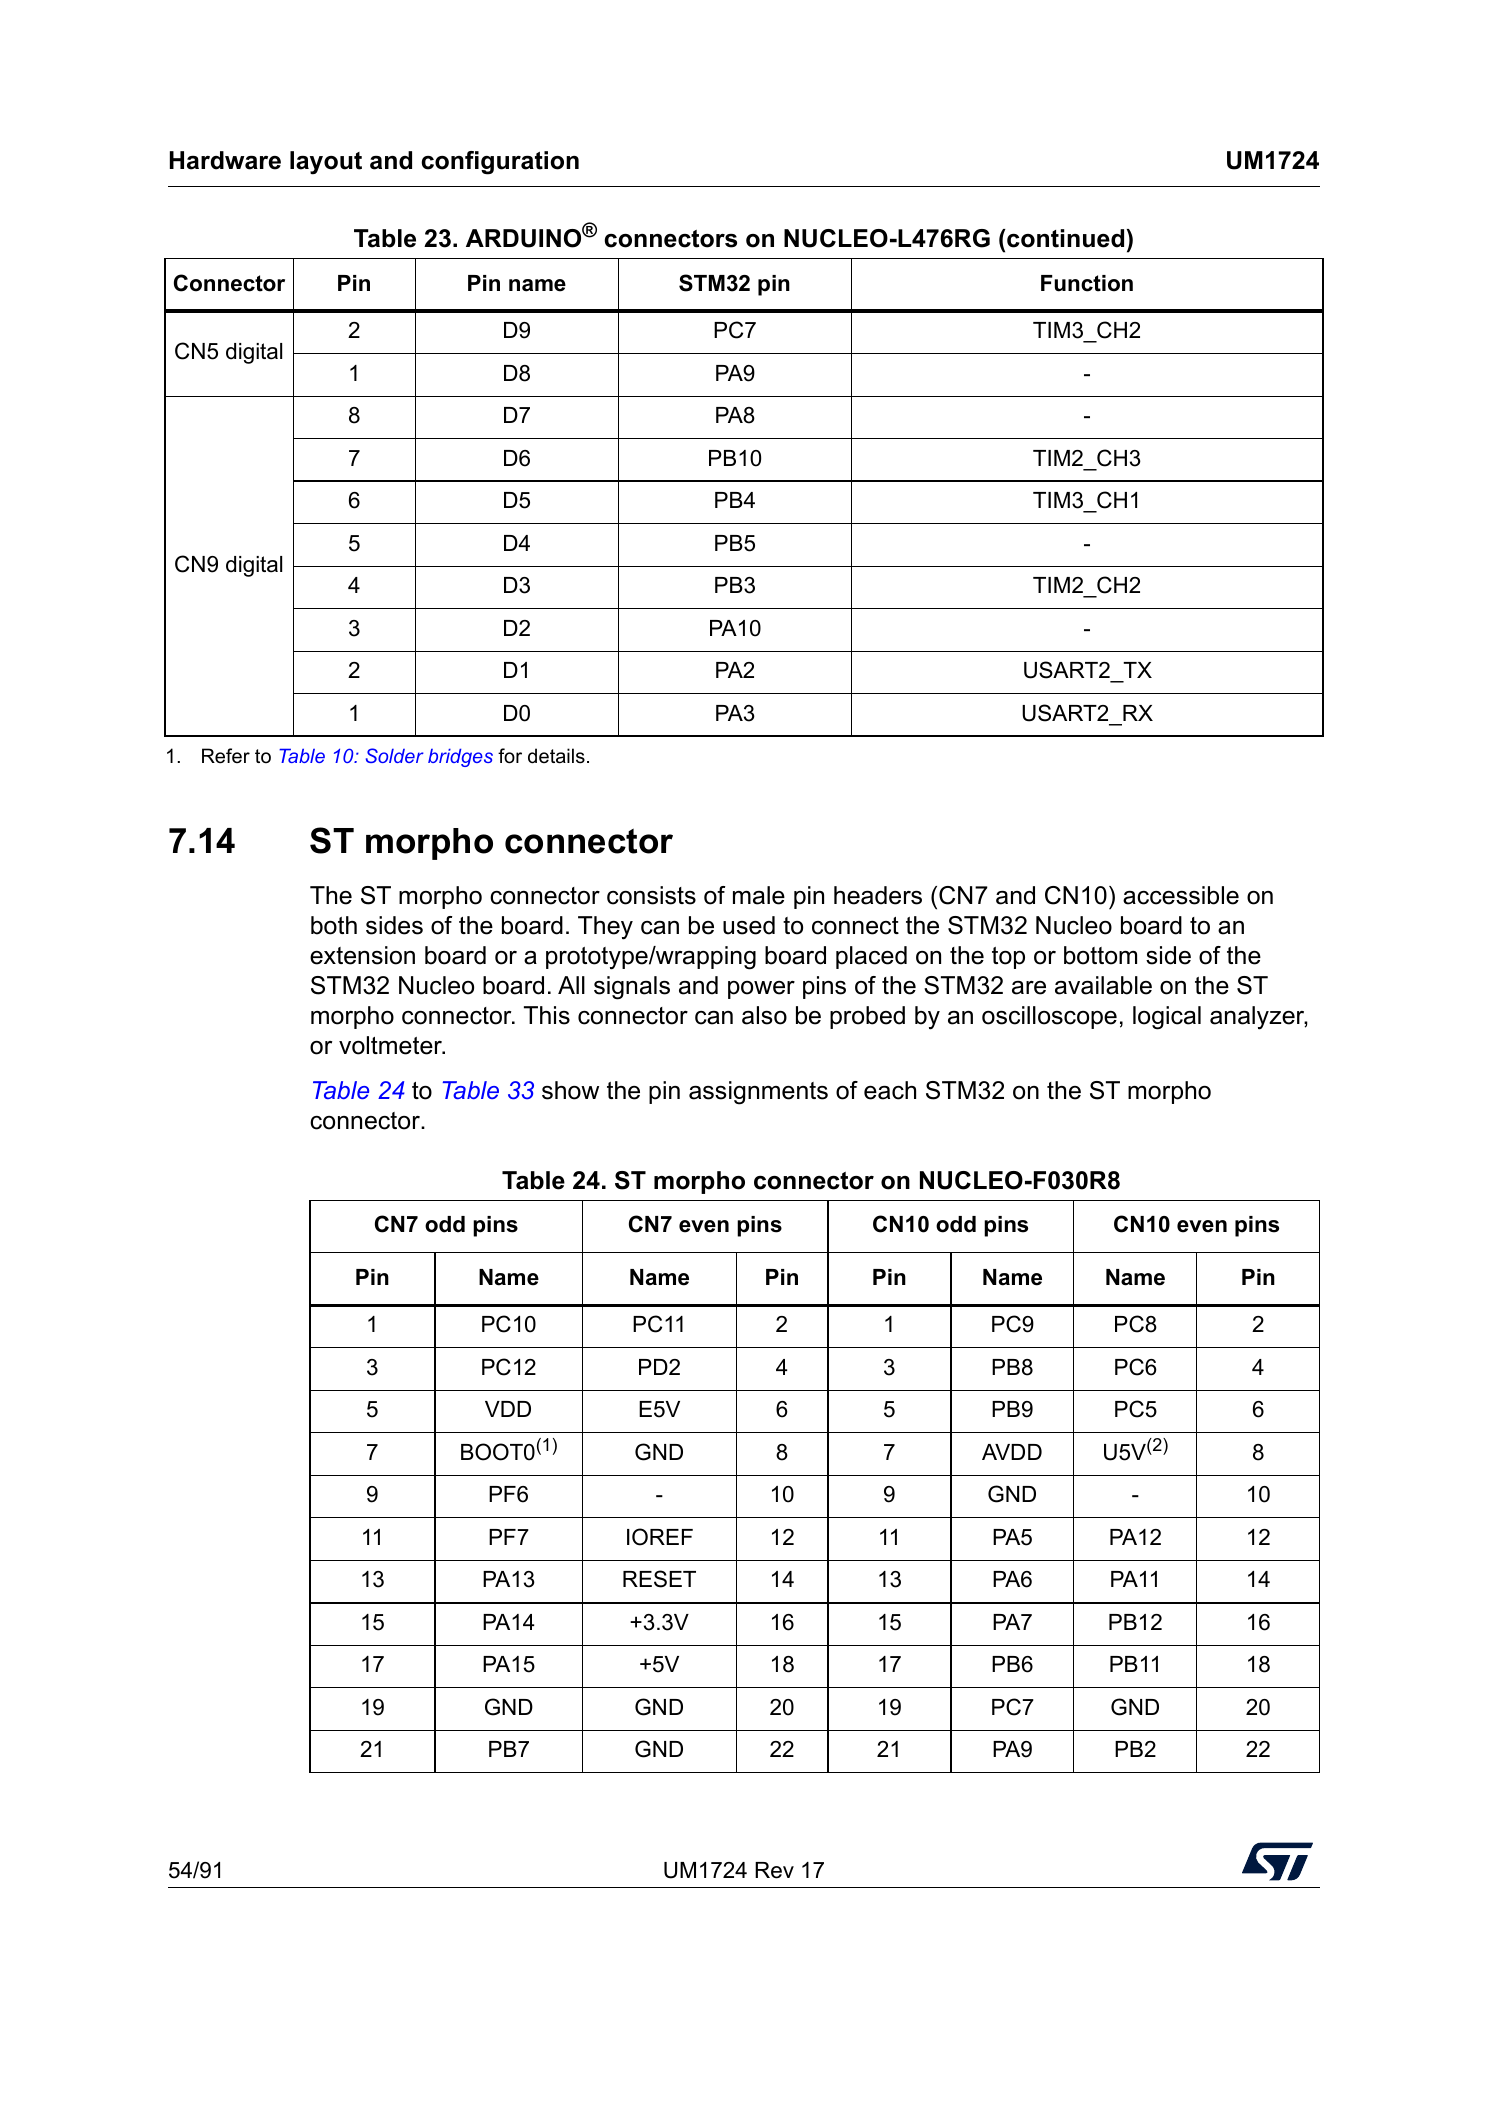
\includegraphics[width=0.94\linewidth]{assets/screenshots/um1724-table23-arduino-connectors-54.png}
\caption{UM1724 page 54, continuation of Table 23. This screenshot shows the
actual firmware pins: D8 maps to PA9, D7 maps to PA8, D4 maps to PB5, and D1
maps to PA2 with USART2\_TX. These are the display data, display clock, display
latch, and serial transmit connections used by the project.}
\label{fig:official-um1724-connector-evidence}
\end{figure}

\subsection{MB1136 Schematic Evidence}

\begin{figure}[H]
\centering
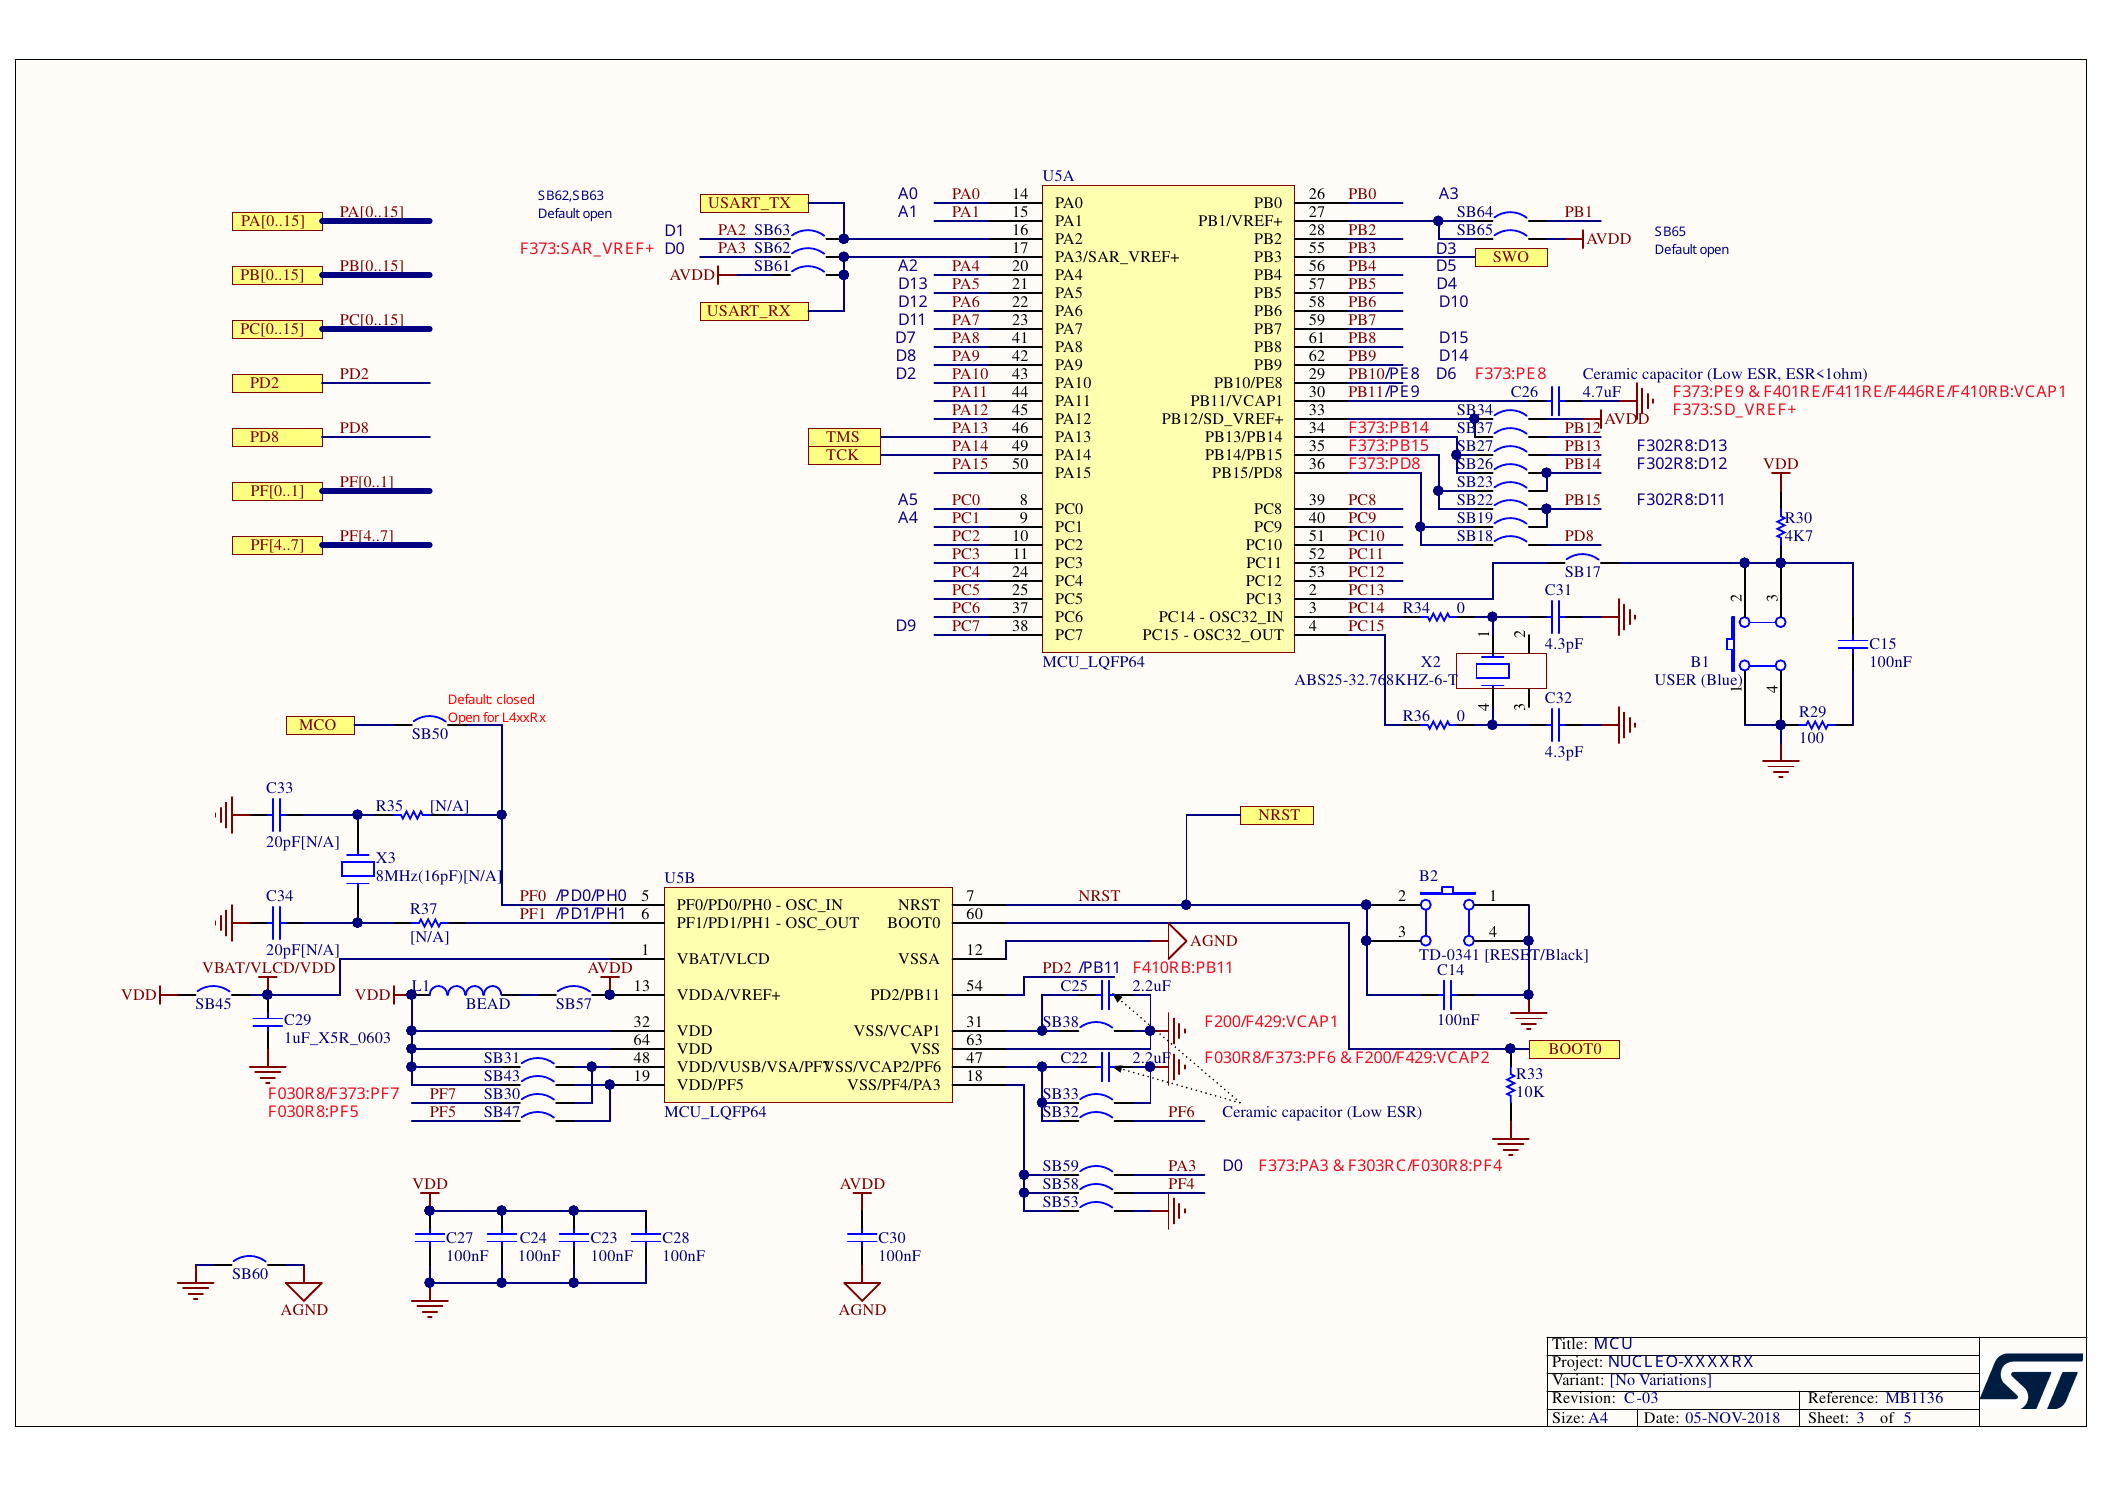
\includegraphics[width=\linewidth]{assets/screenshots/mb1136-sheet3-mcu-3.png}
\caption{MB1136-DEFAULT-C03 schematic, sheet 3 of 5. The MCU sheet shows PA2 on
the USART\_TX path, PA9 on D8, PA8 on D7, PB5 on D4, and VDDA/VREF+ on the
analog supply domain. This confirms the board-level nets that the display and
UART firmware drive.}
\label{fig:official-mb1136-schematic-evidence}
\end{figure}

\subsection{STM32L476xx Internal ADC Evidence}

\begin{figure}[H]
\centering
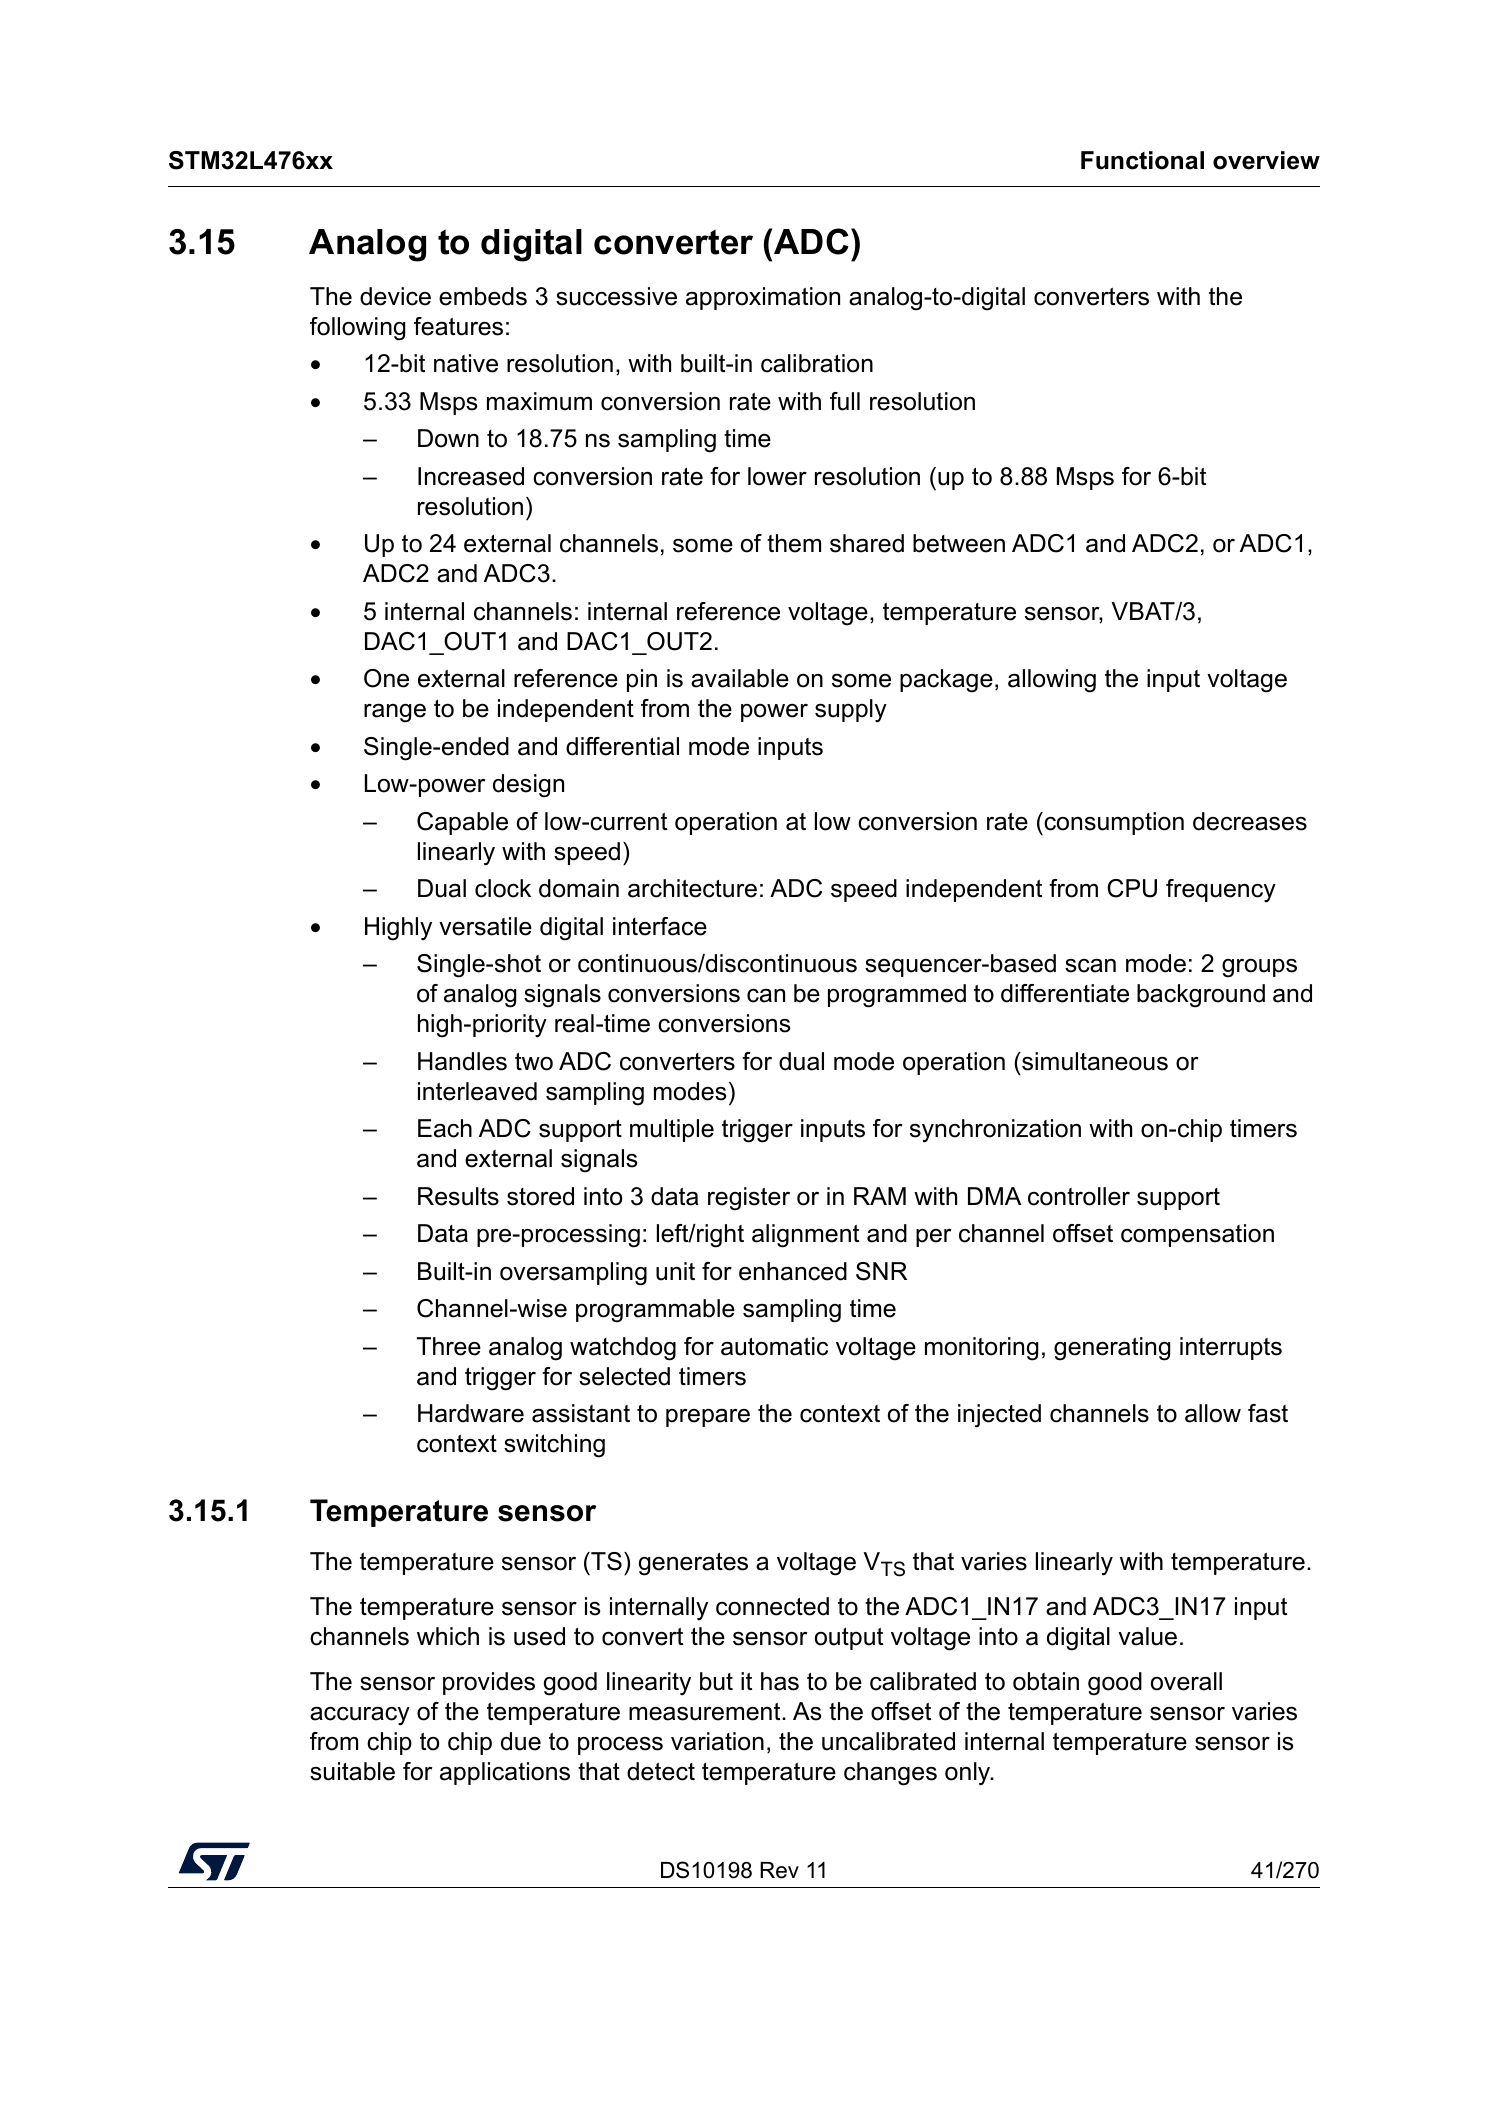
\includegraphics[width=0.94\linewidth]{assets/screenshots/stm32l476-datasheet-temperature-sensor-041.png}
\caption{STM32L476xx datasheet page 41. The ADC functional overview lists the
internal reference and temperature sensor among the ADC internal channels, then
states that the temperature sensor is internally connected to ADC1\_IN17 and
ADC3\_IN17. The firmware uses ADC1 channel 17 for this reading.}
\label{fig:official-l476-temp-sensor-evidence}
\end{figure}

\begin{figure}[H]
\centering
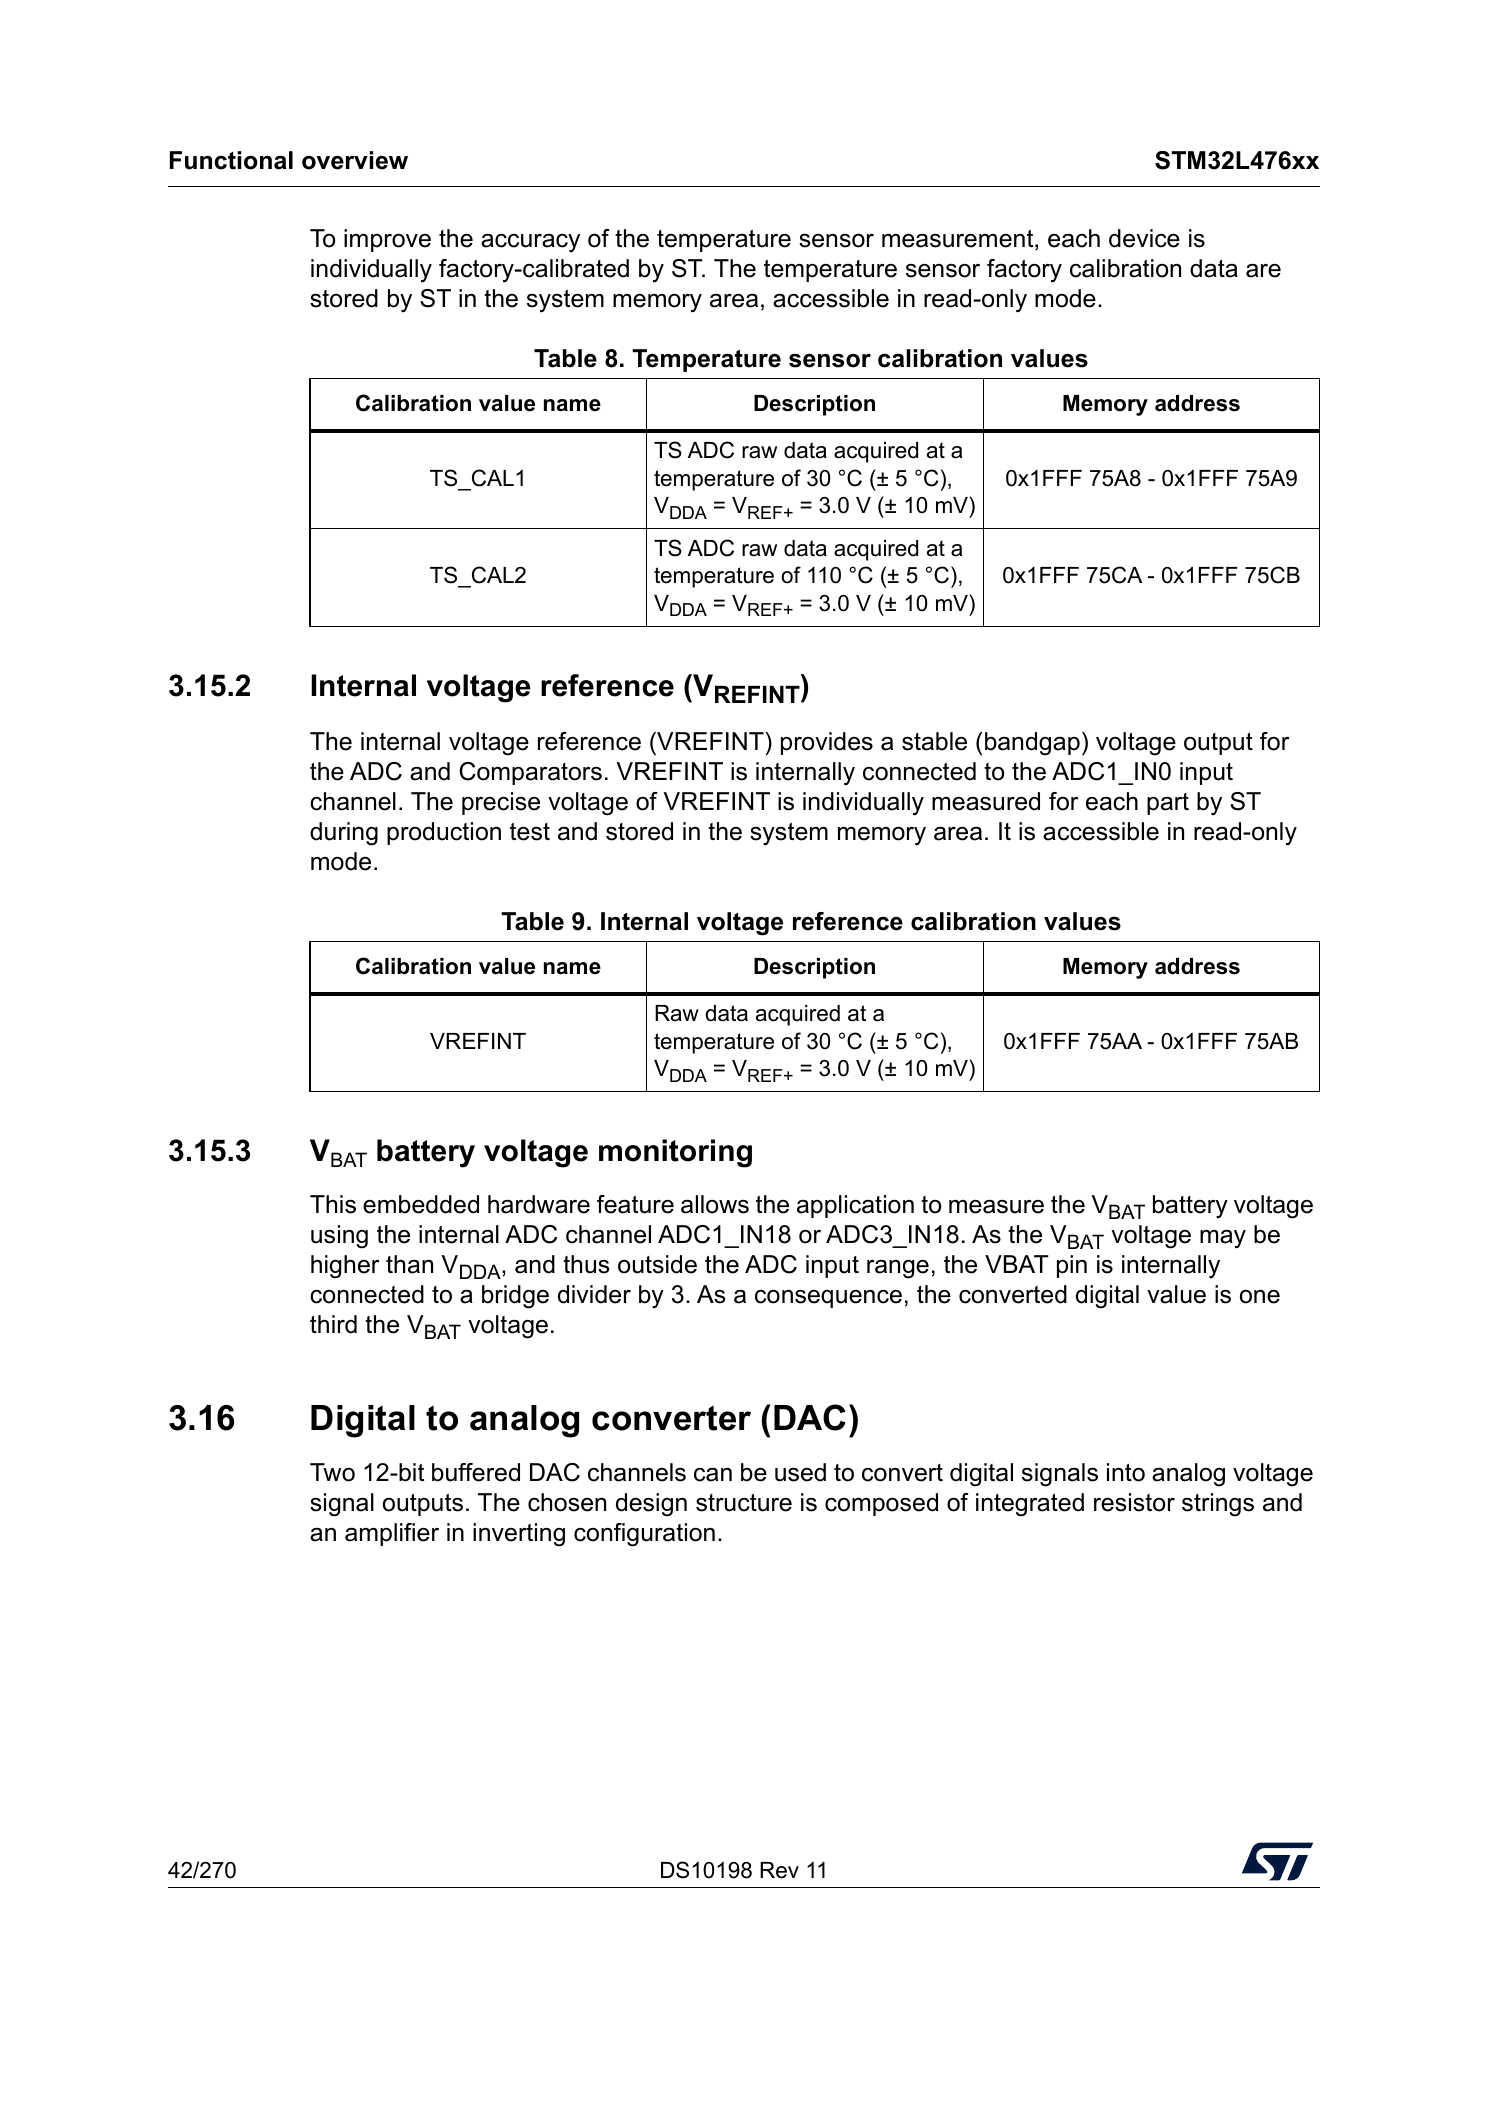
\includegraphics[width=0.94\linewidth]{assets/screenshots/stm32l476-datasheet-adc-internal-042.png}
\caption{STM32L476xx datasheet page 42. This page shows the temperature
calibration words TS\_CAL1 and TS\_CAL2, and states that VREFINT is connected to
ADC1\_IN0. The same page shows the VREFINT calibration word used by the firmware
to estimate VDDA before applying the temperature equation.}
\label{fig:official-l476-adc-evidence}
\end{figure}

\section{System Diagrams}

\subsection{Product Context}

Figure~\ref{fig:product-context} shows the black-box product boundary. The user
only sees power, the display, and the serial diagnostic stream. The temperature
sensor and VREFINT source are internal MCU resources, so the external hardware
contract is small: the Nucleo board, the display shield pins, and the ST-LINK
serial path.

\begin{figure}[H]
\centering
\resizebox{0.94\linewidth}{!}{%
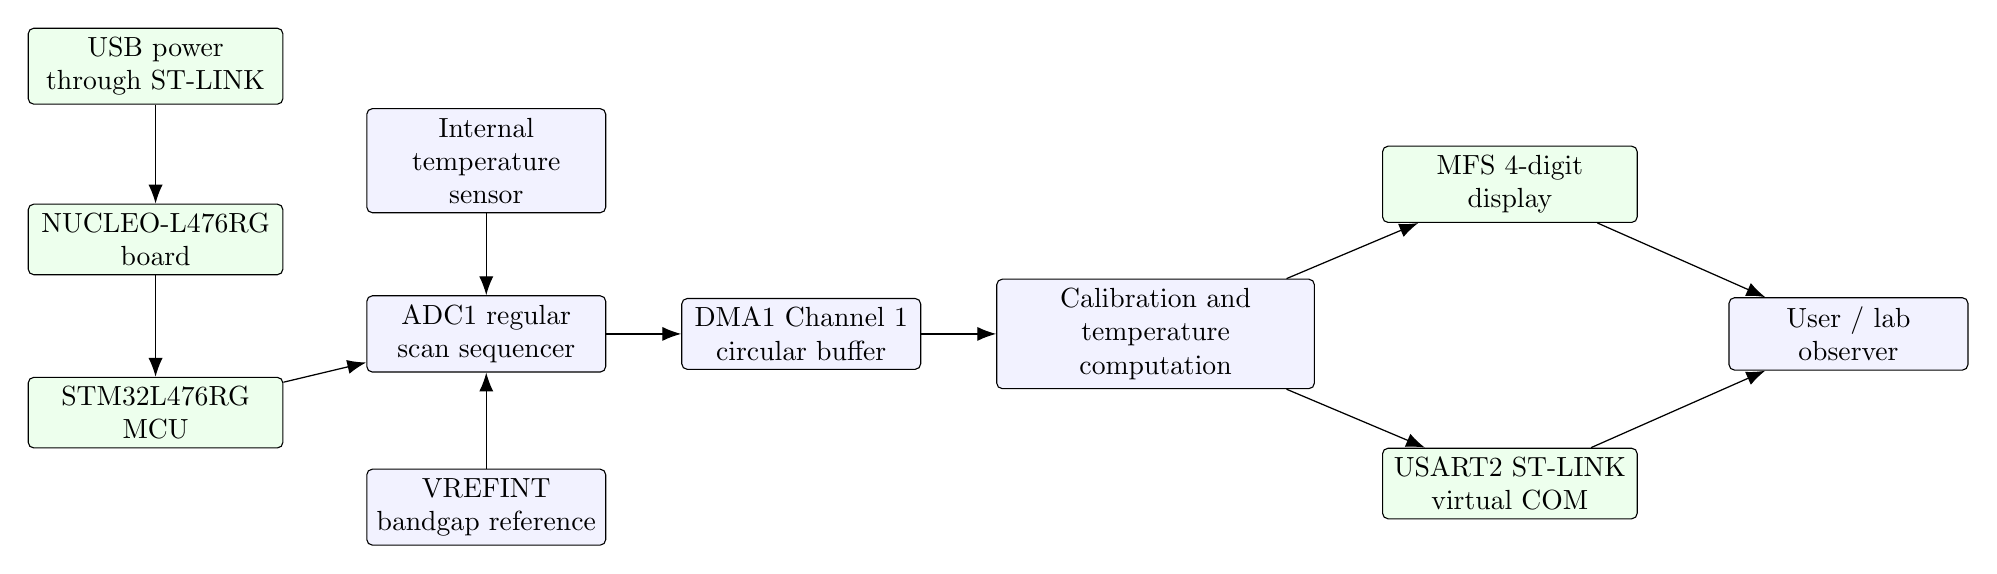
\begin{tikzpicture}[x=1mm,y=1mm]
  \node[hwblock] (power) at (0,22) {USB power\\through ST-LINK};
  \node[hwblock] (board) at (0,0) {NUCLEO-L476RG\\board};
  \node[hwblock] (mcu) at (0,-22) {STM32L476RG\\MCU};

  \node[block] (ts) at (42,10) {Internal\\temperature sensor};
  \node[block] (vref) at (42,-34) {VREFINT\\bandgap reference};
  \node[block] (adc) at (42,-12) {ADC1 regular\\scan sequencer};
  \node[block] (dma) at (82,-12) {DMA1 Channel 1\\circular buffer};
  \node[wideblock] (math) at (127,-12) {Calibration and\\temperature computation};

  \node[hwblock] (display) at (172,7) {MFS 4-digit\\display};
  \node[hwblock] (serial) at (172,-31) {USART2 ST-LINK\\virtual COM};
  \node[block] (user) at (215,-12) {User / lab observer};

  \path (power) edge (board)
        (board) edge (mcu)
        (mcu) edge (adc)
        (ts) edge (adc)
        (vref) edge (adc)
        (adc) edge (dma)
        (dma) edge (math)
        (math) edge (display)
        (math) edge (serial)
        (display) edge (user)
        (serial) edge (user);
\end{tikzpicture}%
}
\caption{Product-level context from power input to human-visible outputs.}
\label{fig:product-context}
\end{figure}

\subsection{ADC and DMA Pipeline}

Figure~\ref{fig:adc-dma-pipeline} shows the measurement path implemented in
\texttt{temp\_sensor.c}. Initialization prepares the ADC regulator, common ADC
internal channels, self-calibration, DMA, and regular scan sequence. Runtime
data then flows from ADC1 into the circular DMA buffer, through averaging, VDDA
estimation, temperature interpolation, and finally to the display and UART
reporting paths. ADC overrun and DMA transfer errors bypass the normal valid
snapshot path and are surfaced as fault states.

\begin{figure}[H]
\centering
\resizebox{0.98\linewidth}{!}{%
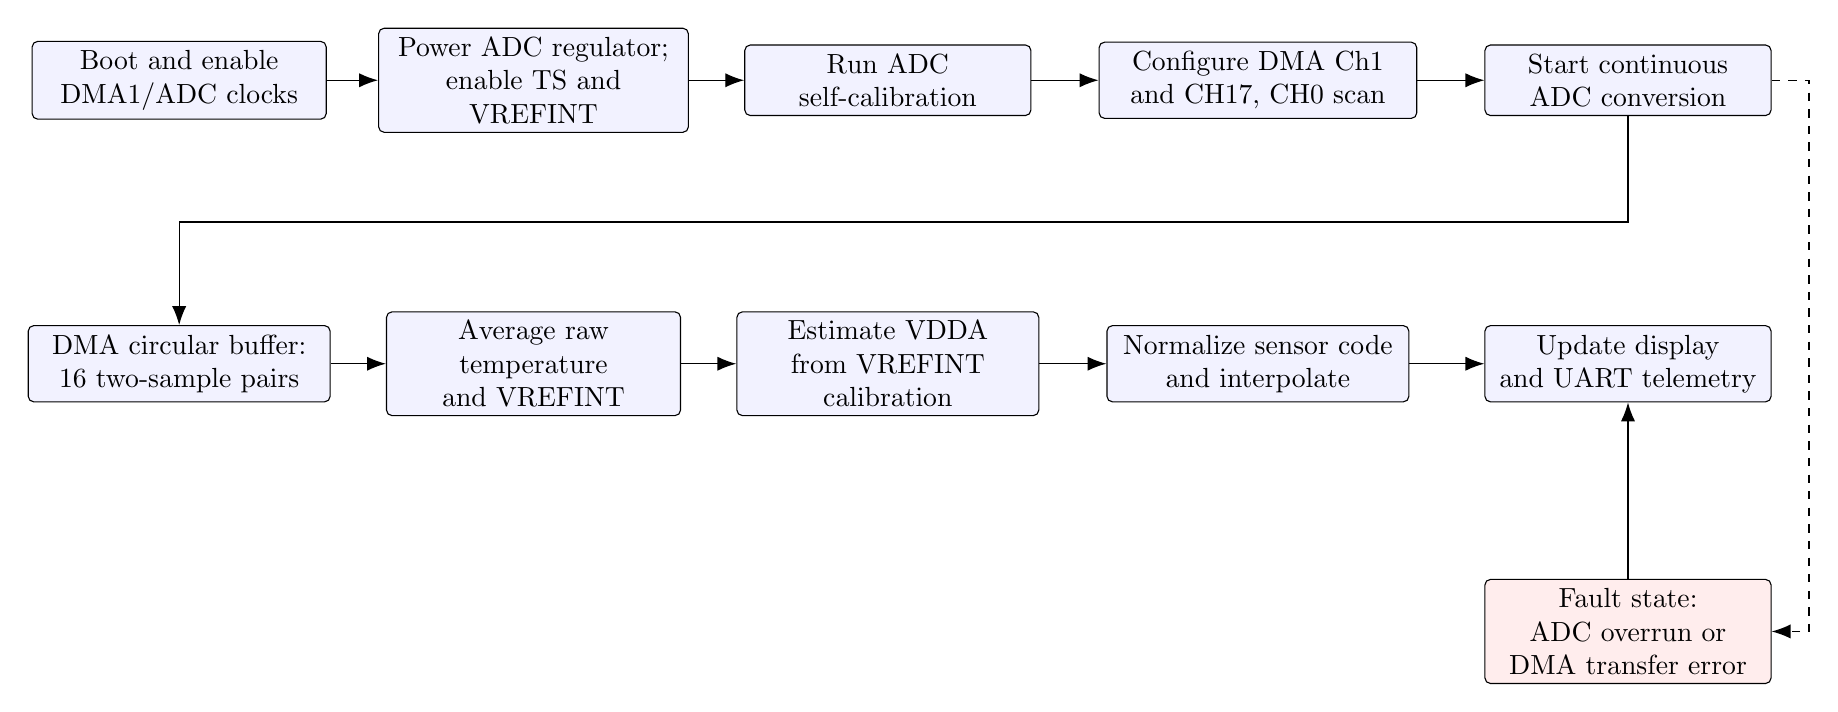
\begin{tikzpicture}[x=1mm,y=1mm]
  \node[wideblock, text width=35mm] (boot) at (0,12) {Boot and enable\\DMA1/ADC clocks};
  \node[wideblock, text width=37mm] (analog) at (45,12) {Power ADC regulator;\\enable TS and VREFINT};
  \node[wideblock, text width=34mm] (cal) at (90,12) {Run ADC\\self-calibration};
  \node[wideblock, text width=38mm] (cfg) at (137,12) {Configure DMA Ch1\\and CH17, CH0 scan};
  \node[wideblock, text width=34mm] (start) at (184,12) {Start continuous\\ADC conversion};

  \node[wideblock, text width=36mm] (buf) at (0,-24) {DMA circular buffer:\\16 two-sample pairs};
  \node[wideblock, text width=35mm] (avg) at (45,-24) {Average raw\\temperature and VREFINT};
  \node[wideblock, text width=36mm] (vdda) at (90,-24) {Estimate VDDA\\from VREFINT calibration};
  \node[wideblock, text width=36mm] (temp) at (137,-24) {Normalize sensor code\\and interpolate};
  \node[wideblock, text width=34mm] (out) at (184,-24) {Update display\\and UART telemetry};
  \node[faultblock, text width=34mm] (fault) at (184,-58) {Fault state:\\ADC overrun or\\DMA transfer error};

  \path (boot) edge (analog)
        (analog) edge (cal)
        (cal) edge (cfg)
        (cfg) edge (start)
        (buf) edge (avg)
        (avg) edge (vdda)
        (vdda) edge (temp)
        (temp) edge (out)
        (fault) edge (out);
  \draw[-{Latex[length=2.4mm]}, line width=0.45pt]
        (start.south) -- (184,-6) -- (0,-6) -- (buf.north);
  \draw[-{Latex[length=2.4mm]}, dashed, line width=0.45pt]
        (start.east) -- (207,12) -- (207,-58) -- (fault.east);
\end{tikzpicture}%
}
\caption{ADC1, DMA1 Channel 1, calibration, and output pipeline.}
\label{fig:adc-dma-pipeline}
\end{figure}

\subsection{Firmware Timing}

Figure~\ref{fig:firmware-timing} summarizes the cooperative timing model. The
SysTick interrupt owns the millisecond counter; the foreground loop checks
elapsed time and performs short scheduled actions. Display multiplexing runs
every 2 ms, display text updates every 250 ms, and serial diagnostics run every
1000 ms. Between checks, the firmware waits for interrupt with \texttt{\_\_WFI()}.

\begin{figure}[H]
\centering
\resizebox{0.90\linewidth}{!}{%
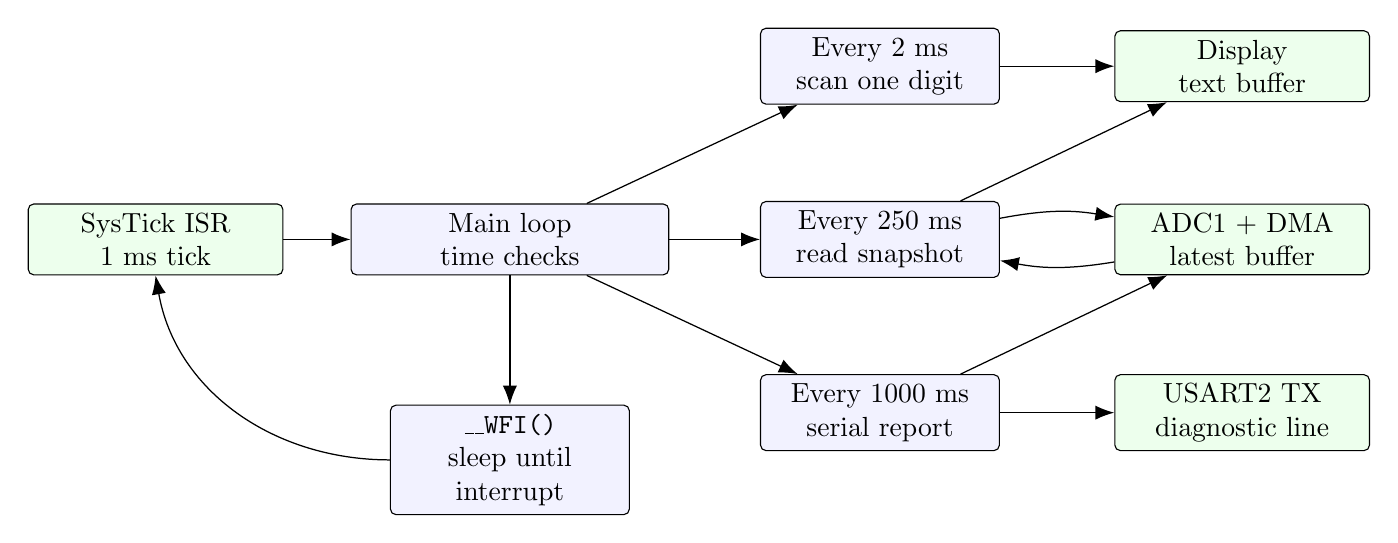
\begin{tikzpicture}[x=1mm,y=1mm]
  \node[hwblock] (systick) at (0,0) {SysTick ISR\\1 ms tick};
  \node[wideblock] (main) at (45,0) {Main loop\\time checks};
  \node[block] (wfi) at (45,-28) {\texttt{\_\_WFI()}\\sleep until interrupt};

  \node[block] (displayfast) at (92,22) {Every 2 ms\\scan one digit};
  \node[block] (adc250) at (92,0) {Every 250 ms\\read snapshot};
  \node[block] (uart1000) at (92,-22) {Every 1000 ms\\serial report};

  \node[hwblock] (display) at (138,22) {Display\\text buffer};
  \node[hwblock] (adc) at (138,0) {ADC1 + DMA\\latest buffer};
  \node[hwblock] (uart) at (138,-22) {USART2 TX\\diagnostic line};

  \path (systick) edge (main)
        (main) edge (displayfast)
        (main) edge (adc250)
        (main) edge (uart1000)
        (displayfast) edge (display)
        (adc250) edge[bend left=10] (adc)
        (adc) edge[bend left=10] (adc250)
        (adc250) edge (display)
        (uart1000) edge (adc)
        (uart1000) edge (uart)
        (main) edge (wfi)
        (wfi.west) edge[out=180,in=-80] (systick.south);
\end{tikzpicture}%
}
\caption{Foreground timing and interrupt wake-up model.}
\label{fig:firmware-timing}
\end{figure}

\section{Verification Plan}

The expected engineering validation path is:

\begin{enumerate}[leftmargin=*]
  \item Build with PlatformIO using the project environment
        \texttt{nucleo\_l476rg}.
  \item Flash the board over ST-LINK.
  \item Open the virtual COM port at 115200 baud.
  \item Confirm boot line:
\begin{lstlisting}
adc-temp boot: ADC1 channel 17 + VREFINT, DMA1 channel 1 circular
\end{lstlisting}
  \item Confirm repeated \texttt{status=OK} lines with nonzero
        \texttt{raw\_temp}, nonzero \texttt{raw\_vref}, plausible
        \texttt{vdda\_mv}, and plausible room-temperature \texttt{temp\_c}.
  \item Confirm the display shows rounded Celsius and does not remain on
        \texttt{AERR} or \texttt{DERR}.
\end{enumerate}

This documentation package itself is validated by compiling
\texttt{adc-temperature-monitor.tex} with \texttt{pdflatex}.

\section{Known Limits and Engineering Assumptions}

\begin{itemize}[leftmargin=*]
  \item The internal temperature sensor measures MCU die temperature, not ambient
        air temperature.
  \item The conversion assumes the ST factory calibration words are readable and
        valid for the target STM32L476RG device.
  \item The firmware uses integer arithmetic. This is deterministic and small,
        but it truncates intermediate fractional values.
  \item The display is limited to four characters, so the human-facing display
        clamps valid values to -9 through 99 degrees C.
  \item UART transmit is blocking. At one line per second this is acceptable for
        the current product contract.
  \item No hardware-in-the-loop validation is encoded in the repository test
        tree. Board validation remains a manual upload and serial/display check.
\end{itemize}

\section{Appendix: Source Snippets}

\subsection{Snapshot Contract}

\begin{lstlisting}[language=C]
typedef struct {
    uint16_t temp_raw;
    uint16_t vref_raw;
    uint32_t vdda_mv;
    int32_t temp_centi_c;
    bool valid;
    bool adc_fault;
    bool dma_fault;
} temp_sensor_snapshot_t;
\end{lstlisting}

\subsection{Calibration Addresses}

\begin{lstlisting}[language=C]
TS_CAL1_ADDR = 0x1FFF75A8UL
TS_CAL2_ADDR = 0x1FFF75CAUL
VREFINT_CAL_ADDR = 0x1FFF75AAUL
\end{lstlisting}

\subsection{ADC Sequence}

\begin{lstlisting}[language=C]
ADC1->SQR1 = (1UL << ADC_SQR1_L_Pos)
             | (ADC_CHANNEL_TEMPSENSOR << ADC_SQR1_SQ1_Pos)
             | (ADC_CHANNEL_VREFINT << ADC_SQR1_SQ2_Pos);
\end{lstlisting}

\end{document}
